\documentclass[11pt]{article}

\usepackage[T1]{fontenc}
\usepackage{lmodern}
\usepackage[margin=1in,headheight=14pt]{geometry}
\usepackage{microtype}
\usepackage{amsmath,amssymb,amsthm}
\usepackage{graphicx}
\usepackage{booktabs}
\usepackage{enumitem}
\usepackage[dvipsnames]{xcolor}
\usepackage[font=small,labelfont=bf,labelsep=period]{caption}
\usepackage[most]{tcolorbox}
\usepackage{fancyhdr}
\usepackage[colorlinks=true,linkcolor=MidnightBlue,citecolor=MidnightBlue,urlcolor=MidnightBlue]{hyperref}
\usepackage[capitalise,noabbrev]{cleveref}

\definecolor{accent}{HTML}{1F4E9C}
\definecolor{boxbg}{HTML}{F3F6FB}
\definecolor{boxframe}{HTML}{9DB2D8}

\theoremstyle{plain}
\newtheorem{theorem}{Theorem}
\newtheorem{proposition}[theorem]{Proposition}
\theoremstyle{remark}
\newtheorem{remark}[theorem]{Remark}
\newtheorem{example}[theorem]{Example}

\newcommand{\dd}{\mathrm{d}}
\newcommand{\R}{\mathbb{R}}

\newtcolorbox{keybox}[1][]{enhanced, breakable, colback=boxbg, colframe=boxframe,
  boxrule=0.6pt, arc=2pt, left=8pt, right=8pt, top=6pt, bottom=6pt,
  fonttitle=\bfseries\color{accent}, coltitle=accent, colbacktitle=boxbg,
  attach boxed title to top left={xshift=8pt,yshift=-7pt},
  boxed title style={boxrule=0pt, colback=boxbg}, title={#1}}

\pagestyle{fancy}
\fancyhf{}
\renewcommand{\headrulewidth}{0.3pt}
\fancyhead[L]{\small\itshape Spikes become jumps: potential applications}
\fancyhead[R]{\small\itshape MATHDB 354674}
\fancyfoot[C]{\small\thepage}

\setlist{itemsep=2pt,topsep=4pt}

\begin{document}

\thispagestyle{plain}
\begin{center}
  {\LARGE\bfseries Spikes Become Jumps\par}
  \vspace{4pt}
  {\large Potential Applications of a Measure-Valued Limit Theorem\\ for Backward Recurrences\par}
  \vspace{8pt}
  {\normalsize\itshape Companion note to MATHDB 354674 (Principia Fall Competition 2026)\par}
  \vspace{10pt}
  {\normalsize Adib Alqurashi\par}
  {\small King Fahd University of Petroleum and Minerals, Dhahran, Saudi Arabia\par}
  \vspace{2pt}
  {\small November 2026\par}
\end{center}
\vspace{4pt}

\section{Summary}

\begin{keybox}[The message in one sentence]
Pointwise convergence of the coefficients does not control a backward recursion; the
\emph{forcing mass} does. Spikes that move with the discretization become jumps in the limit.
\end{keybox}

\noindent
Many computations run a linear recursion backward from a terminal value. Examples include
backward induction in optimal stopping, discounting in dynamic programming, present values
of cash flows, and backpropagation through a residual network. Each has the form
\begin{equation}\label{eq:rec}
  F_n(k) = G_n(k) + H_n(k)\,F_n(k+1), \qquad F_n(K_n)=\mu_n .
\end{equation}
It is tempting to treat~\eqref{eq:rec} as an Euler scheme for the linear ODE
$y'=-g+hy$, where $g$ and $h$ are the pointwise limits of the scaled coefficients
$g_n(x)=nG_n(\lfloor nx\rfloor)$ and $h_n(x)=n\bigl(1-H_n(\lfloor nx\rfloor)\bigr)$.
Conjecture~1 of Bay\'on et al.~\cite{bayon} asked for exactly this. The Principia
solution~\cite{principia} disproved it, and its discrete part is machine-checked in
Lean~\cite{lean}. The counterexample puts a single unit spike in $G_n$ at the index
$\lfloor n/2\rfloor+1$. Its height $n$ grows while its width $1/n$ shrinks, so $g_n\to 0$
pointwise. Its mass stays equal to~$1$, however, and in the limit it reappears as a jump
of size~$1$ (\cref{fig:ce}).

The companion paper~\cite[Theorem~4]{companion} identifies the correct limit object: the
linear equation driven by the \emph{weak limit of the forcing measures}
$\nu_n=\sum_{k<K_n}G_n(k)\,\delta_{k/n}$. This note asks what that result is good for.
We look inside mathematics (\cref{sec:math}), in scientific machine learning
(\cref{sec:sciml}, the main part) and outside mathematics (\cref{sec:outside}). We then
give a practical checklist (\cref{sec:checklist}) and state the limitations honestly
(\cref{sec:limits}).



\paragraph{The result used throughout.}
Fix $b\in(0,1]$ and integers $K_n\le nb$ with $K_n/n\to b$. Let $F_n$ satisfy~\eqref{eq:rec}
for $0\le k<K_n$, and put $f_n(x)=F_n(\lfloor nx\rfloor)$. Assume:
\begin{enumerate}[label=(A\arabic*),leftmargin=3em]
  \item $h$ is continuous on $[0,b]$ and $\max_{k<K_n}|h_n(k/n)-h(k/n)|\to0$;
  \item $G_n\ge0$ and $\nu_n\to\nu$ weakly on $[0,b]$ (in the sense of~\cite{billingsley});
  \item $\mu_n\to\Theta$.
\end{enumerate}

\begin{theorem}[{\cite[Theorem~4]{companion}}]\label{thm:main}
Under \textup{(A1)--(A3)}, for every $x\in(0,b)$ with $\nu(\{x\})=0$,
\begin{equation}\label{eq:limit}
  f_n(x)\;\longrightarrow\; f(x)=\int_{[x,b]}\Phi(x,s)\,\dd\nu(s)+\Theta\,\Phi(x,b),
  \qquad \Phi(x,s)=\exp\Bigl(-\int_x^s h\Bigr).
\end{equation}
At each atom $c$ of $\nu$, $f$ jumps: $f(c-)-f(c+)=\nu(\{c\})$. Between atoms,
$\dd f=hf\,\dd x-\dd\nu$. If $g_n\to g$ in $L^1$ (for example, pointwise convergence plus
uniform integrability), then $f$ is the solution of $y'=-g+hy$ with $y(b)=\Theta$.
Signed forcing is handled by applying the theorem to the positive and negative parts
separately, which is allowed because~\eqref{eq:rec} is linear; the condition is then that $x$ is
an atom of neither weak limit $\nu^{\pm}$, since cancelling spikes can hide a jump from $\nu$.
\end{theorem}

\begin{remark}[Local version]\label{rem:local}
The value $f_n(x)$ depends only on indices $k\ge\lfloor nx\rfloor$. So if $h$ is singular
at the left end (say $h(x)=1/x$), redefine the coefficients below a fixed $a>0$ so that
$h$ becomes continuous on $[0,b]$. This changes nothing for $x>a$, and~\eqref{eq:limit}
holds on $(a,b)$.
\end{remark}

\begin{figure}[h]
  \centering
  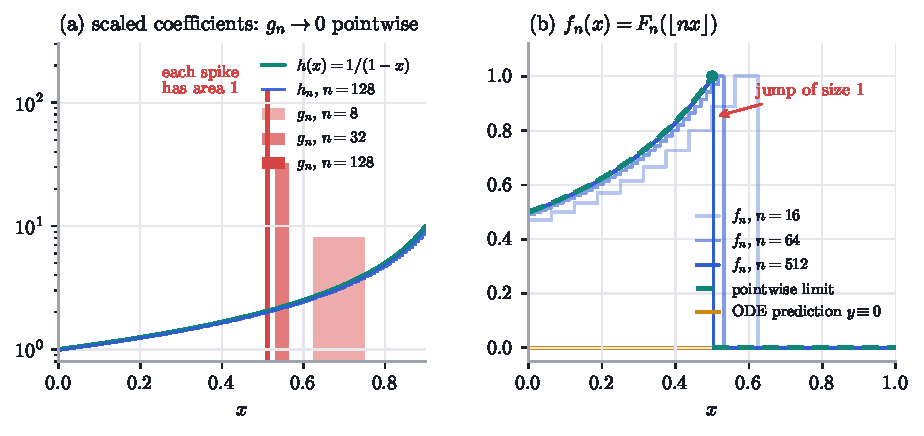
\includegraphics[width=0.94\linewidth]{../figures/paper/fig1_counterexample.pdf}
  \caption{The Principia counterexample~\cite{principia}. (a)~The scaled forcing $g_n$ is
  a spike of height $n$ and area~$1$, so $g_n\to0$ pointwise, while $h_n\to h=1/(1-x)$.
  (b)~The discrete solutions $f_n$ converge to a function with a jump of size~$1$ at $x=1/2$.
  The pointwise-coefficient ODE predicts $y\equiv0$.}
  \label{fig:ce}
\end{figure}

\section{Inside mathematics}\label{sec:math}

\paragraph{(a) Asymptotics of optimal-stopping problems.}
The method of~\cite{bayon} finds asymptotic values of optimal-stopping problems with $n$
candidates. It passes from a backward-induction recurrence to a limiting differential
equation. \Cref{thm:main} lists what has to be checked for that step to be valid.
\begin{example}[Classical secretary problem]
Suppose the first $k$ candidates have been observed, and we then stop at the next relative
best. The success probability $S_n(k)=\tfrac kn\sum_{j=k}^{n-1}\tfrac1j$ satisfies
$S_n(k)=\tfrac1n+\tfrac{k}{k+1}\,S_n(k+1)$ with $S_n(n)=0$. This is~\eqref{eq:rec} with
$G_n\equiv1/n$ and $H_n(k)=k/(k+1)$, so $g\equiv1$ and $h(x)=1/x$. The forcing measures
converge to Lebesgue measure, with no atoms. By \cref{rem:local}, the limit is the ODE
solution $y=-x\ln x$, whose maximum $1/e$ at $x=1/e$ is the classical answer.
\end{example}
Now change the problem so that a fixed payoff is collected at a single decision time
$\lfloor cn\rfloor$, for example a bonus for stopping on a particular interview day.
Then $G_n$ acquires a moving spike. By \cref{thm:main}, the limiting value function jumps
by the limit of that payoff at $x=c$. An ODE built from pointwise limits would miss this
term entirely. So the hypothesis to verify is not ``$g_n\to g$ pointwise'' but
``$\nu_n\to\nu$ weakly'', together with an explicit list of atoms.

\paragraph{(b) Euler-type schemes with rough or impulsive data.}
Read from right to left, \eqref{eq:rec} is an explicit Euler scheme with step $1/n$.
\Cref{thm:main} is a convergence statement for such schemes when the source is a
\emph{measure}, i.e.\ a measure-driven (Stieltjes) linear equation. The forcing may be
smooth, oscillatory, or impulsive, and the only requirement on it is weak convergence. This
is the setting of impulsive control and of ODEs whose sources are point loads or kicks.
For those, a consistency analysis based on pointwise values of the right-hand side is
known to be the wrong test. The result gives a clean, elementary instance of this
principle, with an explicit limit~\eqref{eq:limit}.

\paragraph{(c) The follow-up questions of the Principia solution.}
The solution~\cite{principia} lists four open directions. Their status in the setting of
\cref{thm:main} is:
\begin{center}
\small
\begin{tabular}{@{}p{0.27\linewidth}p{0.64\linewidth}@{}}
\toprule
Direction & Status \\
\midrule
Averaged coefficient control & \emph{Partially answered}: $L^1$ convergence of $g_n$ (e.g.\ pointwise
convergence plus uniform integrability), together with (A1) and (A3), gives the ODE limit with
terminal value $\lim_n F_n(K_n)$; matching it to the conjecture's endpoint selection is still open. \\
Concentrated mass & \emph{Answered for additive spikes}: measure-valued forcing with the jump
rule $f(c-)-f(c+)=\nu(\{c\})$. \\
Endpoint selection & \emph{Open}: the theorem works on $[0,b]$ where $h$ is continuous;
singular endpoints such as $h=1/(1-x)$ at $x=1$ are handled only by restriction. \\
Quantitative rates & \emph{Open}: experiments in~\cite{companion} show $O(1/n)$ away from
atoms, but no rate is proved. \\
\bottomrule
\end{tabular}
\end{center}

\section{Scientific machine learning}\label{sec:sciml}

\paragraph{ResNets are Euler schemes, and backpropagation is a backward recurrence.}
A residual network with $n$ blocks, $z_{k+1}=z_k+\tfrac1n f(z_k,\theta)$, is the explicit
Euler discretization of $\dot z=f(z,\theta)$ on $[0,1]$. This viewpoint was popularized by
E~\cite{e2017} and Haber--Ruthotto~\cite{haber}, and it is the starting point of neural
ODEs~\cite{chen}. Consider a loss with a final term and intermediate terms,
\[
  L=\Psi(z_n)+\sum_m w_m\,\ell_m(z_{k_m}),\qquad k_m/n\to\tau_m\in(0,1).
\]
The backpropagated adjoint $\lambda_k=\partial L/\partial z_k$ satisfies
\begin{equation}\label{eq:adj}
  \lambda_k=\lambda_{k+1}\Bigl(1+\tfrac1n\,\partial_z f(z_k,\theta)\Bigr)
  +\mathbf 1[k=k_m]\,w_m\,\ell_m'(z_k),\qquad \lambda_n=\Psi'(z_n).
\end{equation}
This is exactly~\eqref{eq:rec} with $H_n(k)=1+\partial_z f(z_k)/n$, so
$h(t)=-\partial_z f(z(t),\theta)$. Each intermediate loss contributes a spike of
size $O(1)$ at a depth fraction that moves with $n$.

\begin{proposition}[{\cite[Proposition~10]{companion}}]\label{prop:resnet}
As $n\to\infty$, $\lambda_{\lfloor nt\rfloor}$ converges to the solution of the adjoint
equation $\lambda'=-\partial_z f(z(t),\theta)\,\lambda$, $\lambda(1)=\Psi'(z(1))$,
\emph{with jumps} $\lambda(\tau_m-)-\lambda(\tau_m+)=w_m\,\ell_m'(z(\tau_m))$. Moreover,
$\dd L/\dd\theta\to\int_0^1\lambda(t)\,\partial_\theta f(z(t),\theta)\,\dd t$. Dropping the
jumps (the ``pointwise'' adjoint) leaves an $O(1)$ gradient error that does not vanish as
the depth grows.
\end{proposition}

\paragraph{Why this matters.}
Deep supervision, auxiliary losses on intermediate layers, and latent-ODE models trained
on observations at intermediate times all have the structure of~\eqref{eq:adj}. In their
adjoint method for losses at several observation times, Chen et al.~\cite{chen} integrate
the adjoint backward between observations and update it by the corresponding loss
gradient at each one. \Cref{prop:resnet} explains why that update is necessary and how big
it is: it is exactly the atom of the limiting forcing measure. It also shows what happens
without it. The continuous-depth gradient then disagrees with the gradient that
backpropagation computes in the deep-network limit, so ``optimize-then-discretize'' and
``discretize-then-optimize'' no longer agree.

\begin{figure}[t]
  \centering
  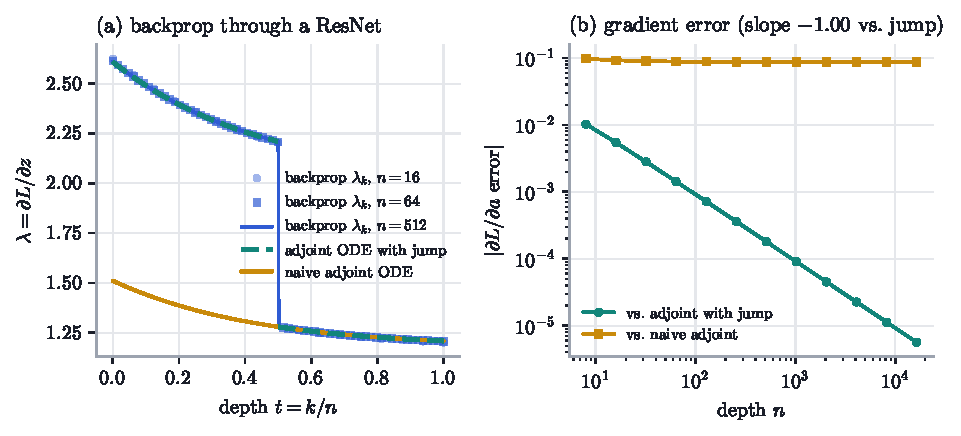
\includegraphics[width=\linewidth]{../figures/paper/fig5_resnet_adjoint.pdf}
  \caption{A scalar $\tanh$ ResNet with an auxiliary loss at the middle layer.
  (a)~Backpropagated adjoints $\lambda_k$ follow the adjoint ODE \emph{with} a jump at
  $t=1/2$, not the naive adjoint. (b)~The gradient error against the jump-aware
  continuous gradient decays like $n^{-1}$. Against the naive adjoint, it stalls at
  $\approx0.087$.}
  \label{fig:adj}
\end{figure}

\paragraph{A numerical check.}
Take $f(z;a,b)=\tanh(az+b)$ with $a=1.3$, $b=0.4$, $z_0=0.5$, final loss
$\tfrac12(z_n-0.2)^2$, and auxiliary loss $\tfrac12 z_{\lfloor n/2\rfloor}^2$ with weight~$1$.
At $n=64$, backpropagation through~\eqref{eq:adj} agrees with central finite differences to
$4.7\times10^{-10}$. \Cref{tab:grad} and \cref{fig:adj} compare the discrete gradient
$\partial L/\partial a$ with the two continuous candidates. The jump-aware value is
$0.266787$, and the discrete gradients converge to it with fitted slope $-1.00$. The naive
adjoint gives $0.180050$, a relative error of about $32\%$ that persists at every depth.

\begin{table}[h]
\centering\small
\caption{Gradient $\partial L/\partial a$ of the ResNet experiment.}\label{tab:grad}
\begin{tabular}{@{}rccc@{}}
\toprule
depth $n$ & backprop $\partial L/\partial a$ & error vs.\ jump-aware & error vs.\ naive \\
\midrule
16    & 0.272237 & $5.45\times10^{-3}$ & $9.22\times10^{-2}$ \\
64    & 0.268212 & $1.42\times10^{-3}$ & $8.82\times10^{-2}$ \\
256   & 0.267147 & $3.60\times10^{-4}$ & $8.71\times10^{-2}$ \\
1024  & 0.266878 & $9.02\times10^{-5}$ & $8.68\times10^{-2}$ \\
4096  & 0.266810 & $2.26\times10^{-5}$ & $8.68\times10^{-2}$ \\
16384 & 0.266793 & $5.64\times10^{-6}$ & $8.67\times10^{-2}$ \\
\midrule
limit & \multicolumn{3}{l}{jump-aware $0.266787$\quad naive $0.180050$\quad ($\approx32\%$ relative error)} \\
\bottomrule
\end{tabular}
\end{table}

\paragraph{Continuous-depth limits of trained networks.}
Cohen, Cont, Rossier and Xu~\cite{cohen} found that the weights of trained deep ResNets
need not converge to a smooth function of depth. Thorpe and van Gennip~\cite{thorpe} study
the deep-layer limit variationally. In both settings, ``the'' continuous model is a choice
of limiting object. \Cref{thm:main} suggests that, at least for the linear backward pass,
measures are the right language. A layer whose contribution stays $O(1)$ while its share of
the depth shrinks shows up as an atom, not as a vanishing density. This is consistent with
those findings rather than a new claim about trained networks. The theorem is scalar, and
we expect the vector case (matrix propagators) to be analogous, but we have not proved it.

\paragraph{Continuous-time reinforcement learning.}
A discounted value recursion $V_k=r_k+\gamma_kV_{k+1}$ with $\gamma_k=1-\rho_k/n$ is again
\eqref{eq:rec}, now with $h=\rho$. When rewards arrive as a rate, $r_k=R(k/n)/n$, the limit
is the familiar continuous-time value
$V(t)=\int_t^{1}e^{-\int_t^s\rho}\,R(s)\,\dd s$ (plus terminal value), as in
Doya's formulation~\cite{doya}. An \emph{impulsive} reward of size $O(1)$ at a time
fraction that moves with the discretization makes $V$ jump by that reward. Temporal-difference
targets computed from a pointwise reward rate would not see it.

\paragraph{PINNs and learned simulators: an analogy.}
Physics-informed neural networks~\cite{raissi} enforce a differential equation through its
residual at collocation points. The analogy with the counterexample is direct: values
sampled at points cannot see mass concentrated between them. If the true source contains
point loads or impulses, the residual must be posed in a weak or measure-aware form, or the
corresponding jump or interface condition must be imposed explicitly. The same applies to
learned time-steppers that are checked by pointwise agreement of their update
coefficients. This is an analogy, not a theorem about PINNs.

\section{Outside mathematics}\label{sec:outside}

The jump rule $f(c-)-f(c+)=\nu(\{c\})$ is classical bookkeeping in several fields. The
interest of \cref{thm:main} there is not novelty. It gives a single statement explaining why
the discrete and continuous models agree once lump sums are treated as atoms.
\begin{itemize}[leftmargin=1.4em]
  \item \textbf{Present values and dividends.} The cum-payment value of a cash-flow stream
  satisfies $P_k=c_k+d_kP_{k+1}$, with discount factors $d_k$. Coupons or dividends paid as
  lump sums are spikes, and in the continuous-time limit the price drops by exactly the
  payment at the payment date (the familiar ex-dividend drop). The same structure appears in
  backward induction for derivatives on assets with discrete dividends.
  \item \textbf{Actuarial reserves.} Prospective reserves of life-insurance contracts obey a
  backward recursion: discounting and survival play the role of $H$, while premiums and
  benefits play the role of $G$. In continuous time this becomes Thiele's differential
  equation, and lump-sum payments make the reserve jump at the payment dates. Our result is
  consistent with this classical picture.
  \item \textbf{Dynamic programming in operations research.} Any finite-horizon linear
  policy evaluation with per-period costs and discounting fits~\eqref{eq:rec}. One-off
  costs (a setup cost, a penalty at a deadline) must be modelled as atoms when passing to a
  continuous-time approximation.
\end{itemize}

\section{A practitioner's checklist}\label{sec:checklist}

\begin{keybox}[Does my discretization converge to the ODE I think it does?]
\begin{enumerate}[label=\textbf{\arabic*.},leftmargin=1.6em]
  \item \textbf{Measure masses, not values.} Compute the largest window mass
  $\max_x\nu_n([x-\delta,x+\delta])$ for a few $\delta$ (\cref{fig:mass}b). For a genuine
  density it decays like $\delta$. If it stays bounded away from~$0$ as $\delta\to0$, there is
  a concentrated mass, and pointwise checks of $g_n$ will not reveal it.
  \item \textbf{Locate the atoms that move with $n$.} Their positions $c$ and limiting
  masses $\nu(\{c\})$ determine the jumps of the limit. Spikes at a \emph{fixed} index (or
  any index $j_n$ with $j_n/n\to0$) wash out instead (\cite[Fig.~2]{companion}).
  \item \textbf{Integrate piecewise and add the jumps.} For neural ODEs or latent ODEs with
  intermediate losses or observations, integrate the adjoint backward between atoms, and at
  each atom add $w_m\ell_m'(z(\tau_m))$ (\cref{prop:resnet}).
  \item \textbf{Check the multiplicative part separately.} \Cref{thm:main} assumes
  $h_n\to h$ uniformly. Spikes in $H_n$ itself are not covered (\cref{sec:limits}).
\end{enumerate}
\end{keybox}

\begin{figure}[h]
  \centering
  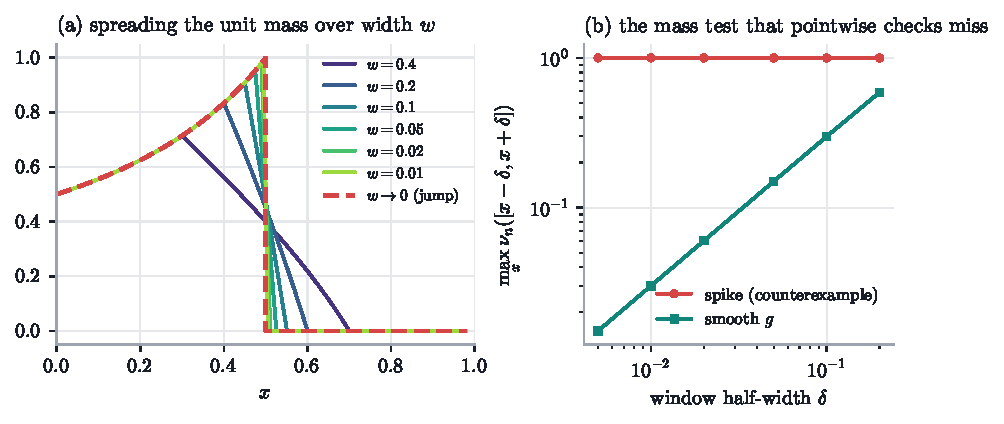
\includegraphics[width=\linewidth]{../figures/paper/fig4_smoothing_and_mass.pdf}
  \caption{(a)~Spreading the unit mass of the counterexample over a window of width $w$
  gives continuous ODE solutions, which sharpen into the jump as $w\to0$. (b)~The
  window-mass diagnostic: it stays equal to~$1$ for the spike but decays linearly in
  $\delta$ for a smooth forcing.}
  \label{fig:mass}
\end{figure}

\section{Limitations and open directions}\label{sec:limits}

\begin{itemize}[leftmargin=1.4em]
  \item \textbf{Uniform convergence of $h_n$.} \Cref{thm:main} requires
  $h_n\to h$ uniformly on $[0,b]$, with $h$ continuous there. Endpoint singularities such as
  $h(x)=1/(1-x)$ at $x=1$ (the case of the counterexample) are handled only by restricting
  to $[0,b]$ with $b<1$. The endpoint-selection question of~\cite{principia} remains open.
  \item \textbf{Multiplicative spikes.} If $H_n$ itself has a spike, e.g.\ $H_n(j_n)=1/2$
  as in the variant in~\cite{principia}, then $h_n$ does not converge uniformly and the
  theorem does not apply. Such spikes should produce \emph{multiplicative} jumps in the
  propagator $\Phi$. A theorem covering them, with $h\,\dd x$ also replaced by a measure, is
  a natural next step.
  \item \textbf{Rates.} The numerics in~\cite{companion} show errors of order $1/n$ away
  from atoms, both for the counterexample and for a generic test with smooth forcing and two
  moving spikes, but no quantitative bound is proved.
  \item \textbf{Scope of the applications.} The SciML and finance statements above are either
  direct corollaries in the scalar linear setting (\cref{prop:resnet}) or analogies that we
  flag as such. They are not claims about the training dynamics of real networks.
\end{itemize}

\begin{thebibliography}{99}\small
\bibitem{bayon}
L.~Bay\'on, P.~Fortuny Ayuso, J.~M.~Grau, A.~M.~Oller-Marc\'en, and M.~M.~Ruiz,
\emph{A new method for computing asymptotic results in optimal stopping problems},
Bull.\ Malays.\ Math.\ Sci.\ Soc.\ \textbf{46} (2023), article~46.
\href{https://doi.org/10.1007/s40840-022-01436-4}{doi:10.1007/s40840-022-01436-4}.

\bibitem{principia}
Principia Math in Progress, \emph{A bounded counterexample to pointwise convergence for
recurrence-defined functions}, MathDB problem 354674, 2026.
\url{https://mathdb.com/p/354674}.

\bibitem{lean}
PrincipiaMathOrg, Lean formalization of MathDB problem 354674,
\url{https://github.com/PrincipiaMathOrg/math-solutions/blob/main/mathdb/Principia/MathDB/Problem354674.lean}.

\bibitem{companion}
A.~Alqurashi, \emph{Moving spikes and measure-valued limits of backward recurrences, with an application to backpropagation through residual networks}, Principia project MathDB 354674, 2026.
Companion paper, Principia project MATHDB 354674.

\bibitem{e2017}
W.~E, \emph{A proposal on machine learning via dynamical systems},
Commun.\ Math.\ Stat.\ \textbf{5} (2017), 1--11.

\bibitem{haber}
E.~Haber and L.~Ruthotto, \emph{Stable architectures for deep neural networks},
Inverse Problems \textbf{34} (2018), 014004.

\bibitem{chen}
R.~T.~Q.~Chen, Y.~Rubanova, J.~Bettencourt, and D.~Duvenaud,
\emph{Neural ordinary differential equations}, Advances in Neural Information Processing
Systems~31 (NeurIPS 2018).

\bibitem{cohen}
A.-S.~Cohen, R.~Cont, A.~Rossier, and R.~Xu, \emph{Scaling properties of deep residual
networks}, Proceedings of the 38th International Conference on Machine Learning
(ICML 2021), PMLR~139.

\bibitem{thorpe}
M.~Thorpe and Y.~van Gennip, \emph{Deep limits of residual neural networks},
Res.\ Math.\ Sci.\ \textbf{10} (2023), article 6.

\bibitem{doya}
K.~Doya, \emph{Reinforcement learning in continuous time and space},
Neural Comput.\ \textbf{12} (2000), no.~1, 219--245.

\bibitem{raissi}
M.~Raissi, P.~Perdikaris, and G.~E.~Karniadakis, \emph{Physics-informed neural networks: a
deep learning framework for solving forward and inverse problems involving nonlinear partial
differential equations}, J.\ Comput.\ Phys.\ \textbf{378} (2019), 686--707.

\bibitem{billingsley}
P.~Billingsley, \emph{Convergence of Probability Measures}, 2nd ed., Wiley, New York, 1999.
\end{thebibliography}

\end{document}
